%%%%%%%%%%%%%%%%%%%
%%% 2023-05-04 %%%%
%%%%%%%%%%%%%%%%%%%
\section{Manipulación (2023-05-04)}

\begin{frame}\frametitle{Posición y Orientación}
  Un cuerpo rígido en el espacio puede tener una posición $(x,y,z)$ y una orientación. La orientación se puede representar de varias formas:
  \begin{itemize}
  \item Mediante ángulos de Euler: roll, pich y yaw $RPY = (\psi, \theta, \phi)$
  \item Mediante cuaterniones
  \item Mediante una matriz de rotación $R \in SO(3)$
  \end{itemize}
  Los ángulos $RPY$ son rotaciones intrínsecas sobre los ejes $X$, $Y$, y $Z$ respectivamente. Se llaman intrínsecas porque son rotaciones que ocurren sobre un sistema de referencia \textit{atado} a un cuerpo rígido.\\
  Cualquier orientación se puede obtener mediante la composición de tres rotaciones básicas:
  \[R = R_{z,\phi}R_{y,\theta}R_{x,\psi}\]
  Es decir, primero una rotación de $\phi$ radianes sobre el eje $Z$, seguida de una rotación de $\theta$ radianes sobre el eje $Y$ del sistema resultante y una rotación de $\psi$ radianes sobre el eje $X$ del sistema rotado. 
\end{frame}

\begin{frame}\frametitle{Transformaciones Homogéneas}
  Una Transformación Homogénea es una matriz de la forma
  \[T = \left[\begin{tabular}{cccc}
      & & & $d_x$\\
      & $R\in SO(3)$ & & $d_y$\\
      & & & $d_z$\\
      0 & 0& 0 & 1
    \end{tabular}\right]\]
  Puede servir para
  \begin{itemize}
  \item Representar la posición y orientación de un cuerpo rígido
  \item Representar una transformación de coordenadas $T_{ab}$ de un sistema de referencia $b$ a un sistema $a$
  \end{itemize}
  Propiedades:
  \begin{itemize}
  \item Asociatividad: $(T_1 T_2) T_3 = T_1 (T_2 T_3)$
  \item Inversa:
    \[T = \left[\begin{tabular}{cc}
       $R^T$ & $-R^T d$\\
       0 & 1
      \end{tabular}\right]\]
  \item Cancelación de índices: $T_{ab} = T_{ac}T_{cb}$
  \end{itemize}
\end{frame}

\begin{frame}\frametitle{El árbol cinemático}
  Es útil tener una descripción de la forma en que están conectadas las diferentes articulaciones del robot. Se considera que sobre cada articulación hay un sistema de referencia (\textit{frame}) que está trasladado y rotado con respecto al sistema anterior.
  \begin{multicols}{3}
    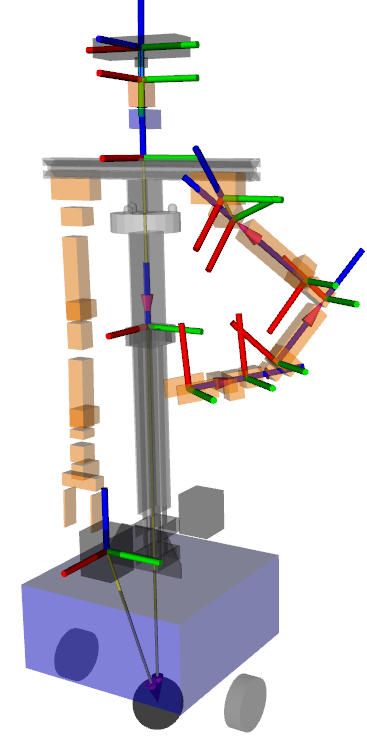
\includegraphics[width=0.26\textwidth]{Figures/KinematicTree.png}\\
    \footnotesize
    El sistema \textit{absoluto} se suele llamar \texttt{map}\\
    El sistema base del robot se suele llamar \textit{base\_link}\\
    Las transformaciones de \texttt{map} a \texttt{base\_link} las determina el sistema de localización\\
    El resto de las transformaciones se determinan con la posición de cada articulación\\
    El árbol cinemático se traduce en una cadena de mulplicaciones de Transformaciones Homogéneas. 
    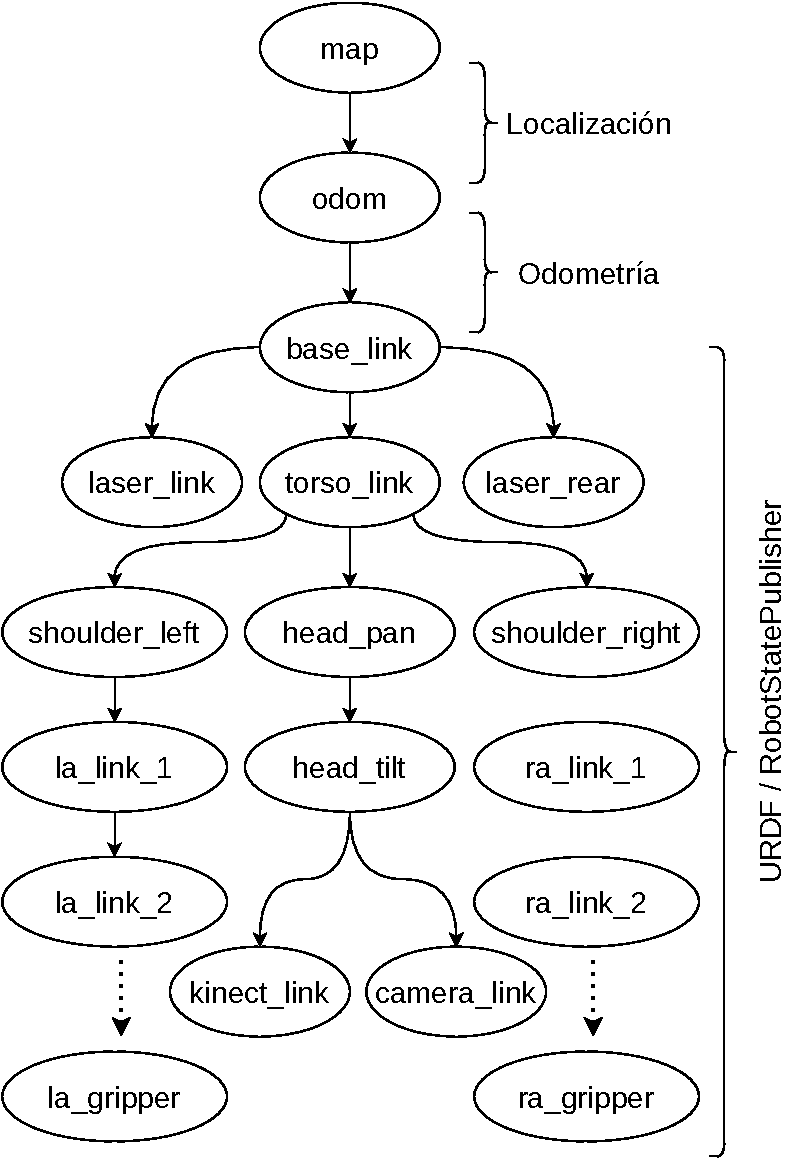
\includegraphics[width=0.35\textwidth]{Figures/TfTree.pdf}
  \end{multicols}
\end{frame}

\begin{frame}[containsverbatim]\frametitle{El formato URDF}
  El formato URDF permite describir el arbol cinemático del robot mediante etiquetas XML:
  \footnotesize
  \lstinputlisting[language=XML]{Codes/URDFExample.xml}
  \normalsize
  Cada etiqueta \texttt{<joint>} representará una Transformación Homogénea. 
\end{frame}

\begin{frame}[containsverbatim]\frametitle{El formato Xacro}
  El formato Xacro es un lenguaje de \textit{macros} que permite obtener archivos XML más cortos. Es últil para especificar parámetros físicos en el URDF como inercias y volúmenes:
  \footnotesize
  \lstinputlisting[language=XML]{Codes/XacroExample.xml}
\end{frame}

\begin{frame}[containsverbatim]\frametitle{Tarea 12 - Transformaciones Homogéneas}
  Abra el archivo \texttt{catkin\_ws/src/hardware/justina\_description/urdf/justina\_base.xacro} y vaya a la línea 228:
  \lstinputlisting[language=XML,firstnumber=227]{Codes/JustinaXacro.xml}
  Modifique el atributo \texttt{xyz} y aumente 1 m en la coordenada en z. Después ejecute el comando:
  \begin{lstlisting}
    roslaunch bring_up path_planning.launch
  \end{lstlisting}
  Detenga la simulación. Ahora modifique el atributo \texttt{rpy}, cambie los valores a ``1.5708 0 0'' y ejecute de nuevo la simulación.
  \begin{itemize}
  \item Observe en el visualizador qué sucede con las lecturas del sensor láser.
  \item Deshaga los cambios. 
  \end{itemize}
\end{frame}

%%%%%%%%%%%%%%%%%%%
%%% 2023-05-09 %%%%
%%%%%%%%%%%%%%%%%%%
\section{Manipulación (2023-05-09)}
\begin{frame}\frametitle{La cinemática directa}
  La cinemática directa consiste en determinar la posición y orientación del efector final del manipulador a partir de la posición de cada articulación.  Esta se puede calcular con la ecuación:
  \[P_1 = T_{12}T_{23}T_{34}T_{45}T_{56}T_{67}T_{7g}P_g\]
  donde $P_g = [0,0,0,1]^T$ es la posición del gripper con respecto al sistema del gripper, $P_1$ es la posición del gripper con respecto al sistema base y $T_{ab}$ es la transformación homogénea que define la rotación y traslación producida por cada articulación. Las matrices $T_{ab}$
  tienen la forma:
  \[T_{ab} = \left[\begin{tabular}{cccc}
      & & & $dx_{ab}$\\
      & $R_{ab}\in SO(3)$ & & $dy_{ab}$\\
      & & & $dz_{ab}$\\
      0 & 0& 0 & 1
    \end{tabular}\right]\]
  Donde $R_{ab}$ representa la rotación del sistema $b$ respecto al sistema $a$ y $(dx_{ab}, dy_{ab}, dz_{ab})$ es la traslación del sistema $b$ respecto al sistema $a$.\\
  La rotación $R_{ab}$ está definida en el URDF por el atributo ``rpy'' de la sub etiqueta \texttt{origin} de la etiqueta \texttt{joint} y por la posición de la articulación. La traslación $(dx_{ab}, dy_{ab}, dz_{ab})$ está definida por el atributo ``xyz''. 
\end{frame}

\begin{frame}\frametitle{Tarea 13 - Cinemática directa}
  
\end{frame}

%%%%%%%%%%%%%%%%%%%
%%% 2023-05-11 %%%%
%%%%%%%%%%%%%%%%%%%
\section{Manipulación (2023-05-11)}
\begin{frame}\frametitle{La cinemática inversa}
  La cinemática inversa consiste en determinar las posiciones que debe tener cada articulación para que el efector final tenga la posición y orientación deseadas.
  \begin{itemize}
  \item Mientras la cinemática directa siempre tiene solución, la cinemática inversa, no.
  \item Se puede resolver por métodos geométricos para obtener una solución cerrada, aunque el análisis puede ser muy complicado.
  \item Una solución más general se puede obtener mediante un método numérico. 
  \end{itemize}
  Suponiendo que se tiene una configuración deseada $p_d \in \mathbb{R}^6$ ($xyz-RPY$), se desea encontrar el conjunto de posiciones articulares $q\in\mathbb{R}^7$ que satisfagan la ecuación
  \[FK(q) - p_d = 0\]
  donde la función $FK$ representa la cinemática directa. 
\end{frame}

\begin{frame}\frametitle{El método Newton-Raphson}
  El método numérico de Newton-Raphson sirve para encontrar raíces, es decir, para resolver ecuaciones de la forma
  \[f(x) = 0\]
  El algoritmo es el siguiente:
  \[\]
  \begin{multicols}{2}
  \begin{algorithm}[H]
    \DontPrintSemicolon
    $x_i \leftarrow x_0$\;
    \While{$|f(x)| > \epsilon$}
    {
       $x_{i+1} \leftarrow x_i - \frac{f(x_i)}{f'(x_i)}$
    }
  \end{algorithm}
  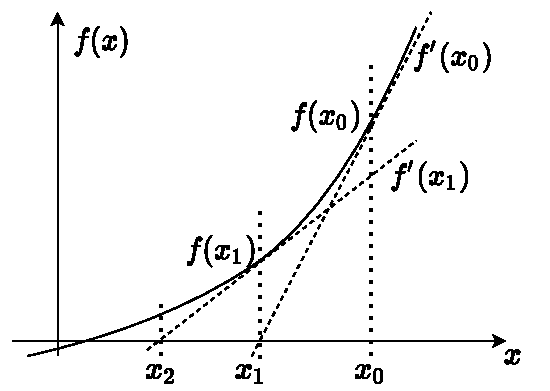
\includegraphics[width=0.4\textwidth]{Figures/NewtonRaphson.pdf}
  \end{multicols}
\end{frame}

\begin{frame}\frametitle{El Jacobiano}
  El Jacobiano es una matriz que relaciona la velocidad articular $\dot{q}$ con la velocidad en el espacio cartesiano $[v\;\omega]^T$ (velocidad lineal y angular):
  \[\dot{p} = \left[\begin{tabular}{c}$v$\\$\omega$\end{tabular}\right] = J \dot{q}
  \qquad\qquad p = [x,y,z,roll, pitch, yaw] \in \mathbb{R}^6, \quad J\in \mathbb{R}^{6\times 7},\quad q\in \mathbb{R}^7\]
  \[J = \left[ \begin{tabular}{ccc}
      $\frac{\partial p_1}{\partial q_1}$ & $\cdots$ & $\frac{\partial p_1}{\partial q_7}$\\
      $\vdots$ & $\ddots$ & $\vdots$ \\
      $\frac{\partial p_6}{\partial q_1}$ & $\cdots$ & $\frac{\partial p_6}{\partial q_7}$\\
    \end{tabular} \right]\]
  \begin{itemize}
  \item La matriz $J$ se puede obtener analíticamente, sin embargo, dado el número de grados de libertad, resulta muy complicado
  \item Se puede obtener aproximando las derivadas parciales con diferencias finitas:
  \end{itemize}
  \[J = \left[\frac{FK(q^1_{+}) -  FK(q^1_{-})}{2\Delta q} \qquad \cdots \qquad \frac{FK(q^7_{+}) -  FK(q^7_{-})}{2\Delta q}\right]\]
  \begin{eqnarray*}
    q^i_+ &=& [q_1\quad \dots \quad q_i + \Delta q \quad \dots \quad q_7]\\
    q^i_- &=& [q_1\quad \dots \quad q_i - \Delta q \quad \dots \quad q_7]
  \end{eqnarray*}
  con $\Delta q$, un valor lo suficientemente pequeño para una buena aproximación de la derivada. 
\end{frame}

\begin{frame}\frametitle{Cinemática Inversa por Newton-Raphson}
  Aplicando Newton-Raphson para resolver la ecuación:
  \[FK(q) - p_d = 0\]
  Se tiene:
  \begin{algorithm}[H]
    \DontPrintSemicolon
    $q_i \leftarrow q_0$ //Una estimación inicial que puede ser la posición articular actual\;
    $p \leftarrow FK(q_i)$ //La posición cartesiana que tendría el gripper con la estimación inicial\;
    \While{$|p - p_d| > \epsilon$}
    {
      $J \leftarrow Jacobiano(q)$     \;
      $q_{i+1} \leftarrow q_i - J^\dagger (p - p_d)$\;
      $p \leftarrow FK(q_i)$ 
    }
  \end{algorithm}
  Puesto que el Jacobiano $J$ no es una matriz cuadrada, no tiene inversa, por lo que se utiliza la matriz pseudoinversa $J^\dagger$. 
  \begin{itemize}
  \item Es importante que las variables angulares siempre estén en el intervalo $(-\pi, \pi]$:
    \begin{itemize}
    \item Las posiciones articulares
    \item Los ángulos roll, pitch, yaw
    \item Las componentes angulares del error $p - p_d$
    \end{itemize}
  \end{itemize}
\end{frame}

\begin{frame}\frametitle{Práctica 10 - Cinemática Inversa}
\end{frame}

%%%%%%%%%%%%%%%%%%%
%%% 2023-05-16 %%%%
%%%%%%%%%%%%%%%%%%%
\section{Manipulación (2023-05-16)}

\begin{frame}\frametitle{Modelo dinámico de un manipulador}
\end{frame}

\begin{frame}\frametitle{Tarea 14 - Modelo dinámico del brazo}
\end{frame}

%%%%%%%%%%%%%%%%%%%
%%% 2023-05-18 %%%%
%%%%%%%%%%%%%%%%%%%
\section{Manipulación (2023-05-18)}

\begin{frame}\frametitle{El control PID}
  El control Proporcional-Integral-Derivativo es un tipo de control lineal en lazo cerrado que calcula la acción de control mediante una combinación lineal del error, la integral del error y la derivada del error.
  \begin{itemize}
  \item Para el manipulador, el ángulo deseado $q_d$ está dado por el resultado de la cinemática inversa. 
  \item La posición angular $q$ se obtiene de los motores o del simulador.
  \item La salida del controlador es el torque $\tau$ que se envía a los motores.
  \end{itemize}
  En la versión continua:
  \[\tau(t) = K_p e(t) + K_I \int e(t)dt + K_d \dot{e}(t)\]
  con $e = q_d - q$
  En la versión discreta:
  \[\tau_i = K_p e_i + K_I\sum_{j=0}^i e_j + K_d\frac{e_i - e_{i-1}}{\Delta t}\]
  con $\Delta t$, el periodo de muestreo. 
\end{frame}

\begin{frame}\frametitle{El control PID}
  Aunque la interacción de las tres señales (error, integral del error y derivada del error) es compleja y depende mucho del sistema, de manera intuitiva se pueden indicar las siguientes funciones de cada componente:
  \begin{itemize}
  \item \textbf{Proporcional:} Aumenta o disminuye el tiempo de asentamiento.
  \item \textbf{Integral:} Reduce el error en estado estable, aunque puede producir inestabiliddad.
  \item \textbf{Derivativa:} Funciona como amortiguamiento y ayuda a disminuir el sobrepaso. 
  \end{itemize}
\end{frame}

\begin{frame}\frametitle{Los \textit{stacks} ros\_control y ros\_controllers}
  Son un conjunto de paquetes que implementan controladores PID y varias interfaces de hardware.
  \begin{itemize}
  \item El stack \texttt{ros\_control} implementa varias interfaces de hardware. En este curso, la interfaz usada es la que interactúa con la simulación de Gazebo. De este stack, el paquete \texttt{controller\_manager} es importante porque utiliza un archivo \textit{yaml} para lanzar otros nodos que implementan controladores PID. 
  \item El stack \texttt{ros\_controllers} implementa varios algoritmos de control para diferentes tipos de actuadores. 
  \end{itemize}
\end{frame}

\begin{frame}\frametitle{Práctia 11 - Control del manipulador}
\end{frame}